\documentclass[aspectratio=169,14pt]{beamer}
\usepackage[utf8]{inputenc}
\usepackage{minted}
\usepackage{listings}
\usetheme{veit}
\title{Memory Vulnerabilities in Memory-safe Languages}
\date{\today}
\author{Veit Heller}
\institute{Information Security Meetup Berlin, August 2020}
\begin{document}
  \maketitle
  \begin{frame}{Python}
    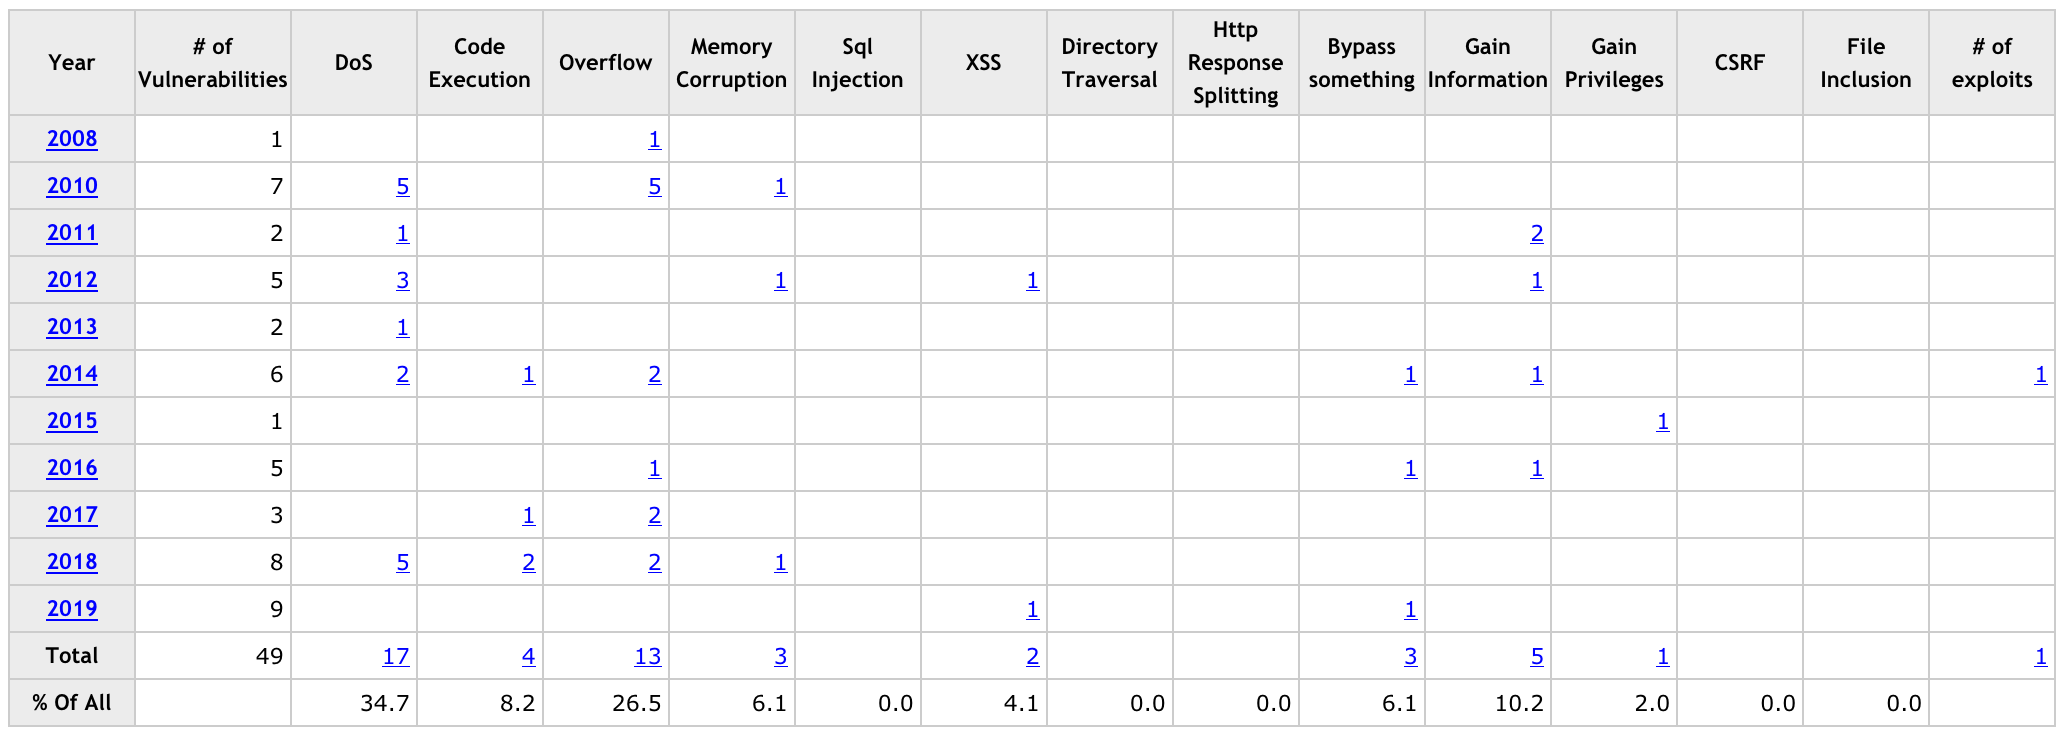
\includegraphics[width=12cm]{python_cves}
  \end{frame}
  \begin{frame}{Space Leaks}
    ``Pinpointing space leaks is a skill that takes practice and perseverance. Better
    tools could significantly simplify the process.``
    --- Mitchell, Neil: Leaking Space. Eliminating memory hogs.
  \end{frame}
  \begin{frame}{References}
    \begin{itemize}
      \item These slides: \texttt{https://github.com/hellerve/talks}
      \item Go bug 20135: \texttt{https://github.com/golang/go/issues/20135}
      \item Breaking Erlang Maps: \texttt{https://medium.com/@jlouis666/breaking-erlang-maps-1-31952b8729e6}
      \item RustBelt: \texttt{https://plv.mpi-sws.org/rustbelt}
      \item Space leak: A Haskell Sore Spot: \texttt{https://fremissant.net/leaky}
      \item Auditing popular Rust crates: how a one-line unsafe has nearly ruined everything: \texttt{https://medium.com/@shnatsel/auditing-popular-rust-crates-how-a-one-line-unsafe-has-nearly-ruined-everything-fab2d837ebb1}
      \item Xu, Hui et al.: Memory-Safety Challenge Considered Solved? An In-Depth Experience Report with All Rust CVEs
      \item Kulal, Sumith et al.: Space leaks exploration in Haskell
      \item Mitchell, Neil: Leaking Space—Eliminating memory hogs
    \end{itemize}
  \end{frame}
  \begin{frame}{}
    Thank you!

    \bigskip

    Questions?
  \end{frame}
\end{document}
